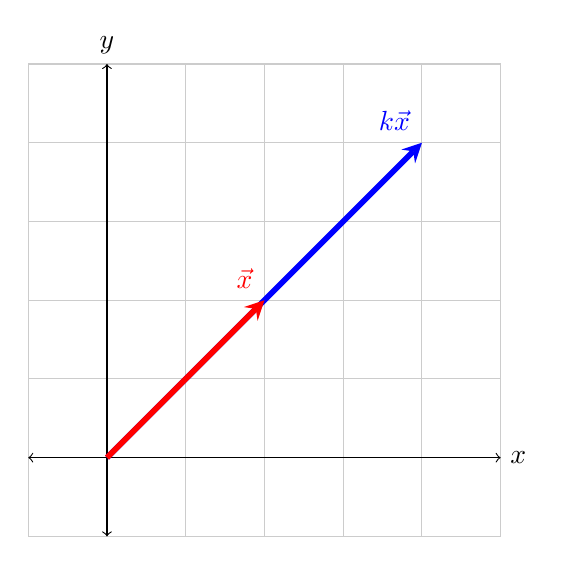
\begin{tikzpicture}
  \draw[thin,gray!40] (-1,-1) grid (5,5); %laver Grid
  \draw[<->] (-1,0)--(5,0) node[right]{$x$}; %x-aksen
  \draw[<->] (0,-1)--(0,5) node[above]{$y$}; %y-aksen
  \draw[line width=2pt,blue,-stealth](0,0)--(4,4) node[above left]{$k\vec{x}$}; %blå vektor
  \draw[line width=2pt,red,-stealth](0,0)--(2,2) node[above left]{$\vec{x}$}; %rød vektor
\end{tikzpicture}
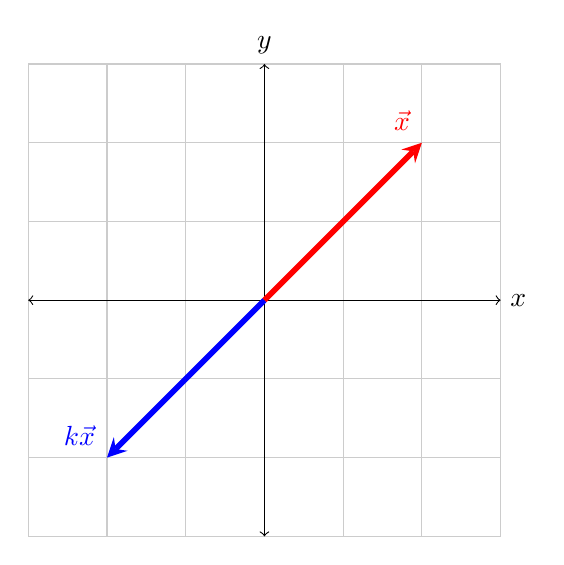
\begin{tikzpicture}
  \draw[thin,gray!40] (-3,-3) grid (3,3);
  \draw[<->] (-3,0)--(3,0) node[right]{$x$};
  \draw[<->] (0,-3)--(0,3) node[above]{$y$};
  \draw[line width=2pt,blue,-stealth](0,0)--(-2,-2) node[above left]{$k\vec{x}$};
  \draw[line width=2pt,red,-stealth](0,0)--(2,2) node[above left]{$\vec{x}$};
\end{tikzpicture}